\title{Computational Modelling in the Humanities and Social Sciences}
\author{mbkb74}
\date{}
\documentclass[12pt]{article}
\usepackage[a4paper, margin=2cm]{geometry}
\usepackage{graphicx}
\usepackage{float}
\usepackage[sorting=none]{biblatex}
\usepackage[parfill]{parskip}
\usepackage{pdfpages}
\addbibresource{bibliography.bib}

\begin{document}
\maketitle

\section{Introduction}

The task I have chosen is to model the features of Castles in England by geographic location. While there were prehistoric hillforts and Roman forts in England prior to this, the main period of castle building in England started after the Battle of Hastings in 1066 \cite{RichardHodges1988OotE}. A popular design of these was the Motte and Bailey castle, with the castle on a raised area of ground (the motte), and a range of supporting buildings protected by a wall (the bailey). The materials used here changed from wood to stone as time went on, which provided much better defence. As the design of the keep was refined, the development then moved onto the outer defences, improving the gatehouses and enclosure walls.

Towards the end of the middle ages, the defence aspect of Castles became less important, and they started to be used as shows of status, with more space, and increasing the size of windows, which reduced the defence, but gave better views.

While I have discussed here the studied aspect of how design has changed with time, there is less information about how design changes with area. Design might change due to the differing requirements of the area, along with differences in geology and geography. As discussed, castles are continually improved, with new designs based on the times, however some castles may have not kept up with these improvements due to the wealth of the owners, or because the castles are left behind.


\section{Sources of data and used modules}

The main source of data will be the National Heritage List for England by Historic England \cite{nhle}. Data will be obtained through this using Beautiful Soup, a web scraping tool for Python \cite{bs}. The data will then be processed by Stanza, a Natural Language Processing Python library \cite{qi2020stanza}. Data is then visualized using plotly in order to make the patterns clearer to see \cite{plotly}.

\section{Models and implementation}

The analysis of text uses multiple of the features from Stanza, first in using Part of Speech Tagging in order to find nouns and plural nouns in the sentences, as these are most likely to be the features I am looking for.

I am also using the provided lemmas feature in order to just extract the singular versions of the nouns, so that if in some cases a feature is discussed in plural, and in some cases singular, they will be treated the same. This has both benefits and drawbacks, providing a benefit in increasing the matching, however the use of the plural may convey information about the features, such as if a castle has multiple towers, compared to one tower.

The dependencies provided are also used to match together compound nouns, such as “curtain wall”, as this provides more information than the separate nouns “curtain” and “wall”.

In order to categorize the castles into sections, I am using NUTS1 regions of England \cite{nuts}, this is an EU specification which divides up countries, in this case, dividing England into 9 regions. There is the option to get more granular with NUTS2 and NUTS3 regions being smaller than NUTS1, however given the limited dataset of around 230 castles, I wanted to ensure there were many castles per region so that the trends would be visible.

The location of each castle is extracted from the webpage, using an Ordnance Survey Grid Reference. This is then turned into latitude and longitude coordinates, which is finally converted into a NUTS region. One area in which this caused some trouble is in castles on small islands, as the converter must have been using a map that excluded these for performance. However the only case in which I discovered this was Lindisfarne castle, so not a significant proportion of the data, and so shouldn't affect the trends seen.

In order to simplify the categorization process, first I ran the code to generate an ordered list of features by how many times they occur. This list was then filtered to just the top 50 that I wanted to observe. This was done to ensure they were significant findings, as if it was just from one castle, it doesn't imply any trend. For these 50 features, a dictionary was created under each NUTS1 region with each features, and as the program went through the castles, the number was incremented if the feature was found in that region. Also kept track of was the total number of castles in each region so that the number of features could be divided by the number of castles to get an average value, ensuring that regions that just had more castles didn't look like they had more of a certain feature.


\section{Evaluation of models}

On evaluating the heatmaps, features did come out as showing as more prominent from certain areas, they can be shown below. You will see that London is white on this map as none of the castles in the dataset were in the London area.

The simplest evaluation of these results is to look at the description of building materials. Due to the difficulty of transportation at the time castles were being built, they use materials from the local area, and so they reflect geological surveys.

The most obvious of these are sandstone, limestone and flint, as shown below



\begin{minipage}{0.45\textwidth}
	\begin{figure}[H]
		\centering
		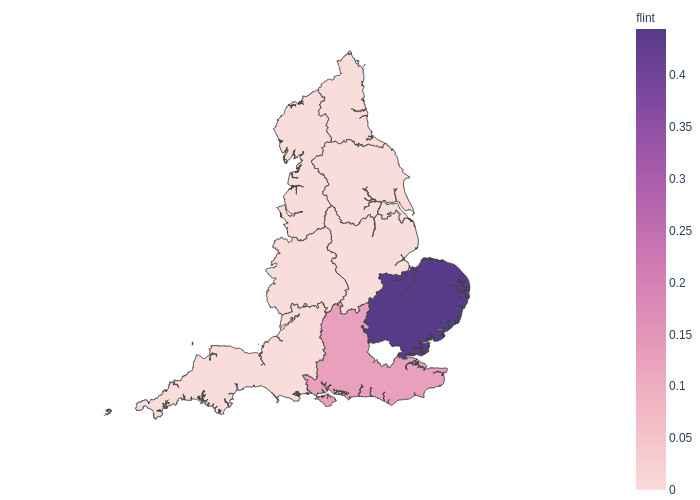
\includegraphics[width=\textwidth]{flint.png}
		\caption{Flint}
	\end{figure}
\end{minipage}
\begin{minipage}{0.45\textwidth}
	\begin{figure}[H]
		\centering
		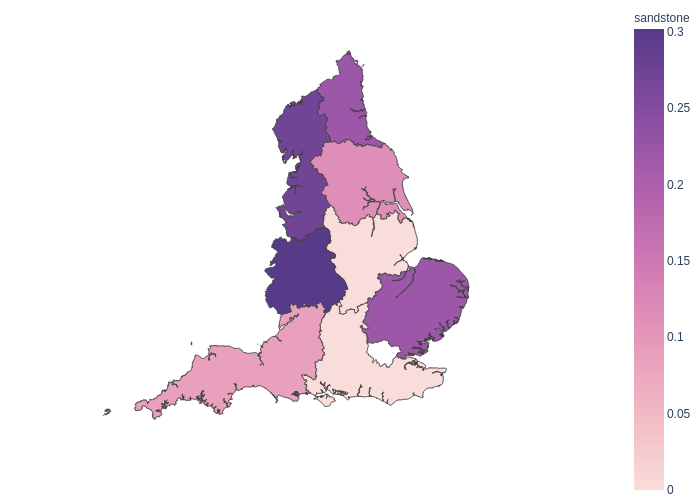
\includegraphics[width=\textwidth]{sandstone.png}
		\caption{Sandstone}
	\end{figure}
\end{minipage}
\begin{figure}[H]
	\centering
	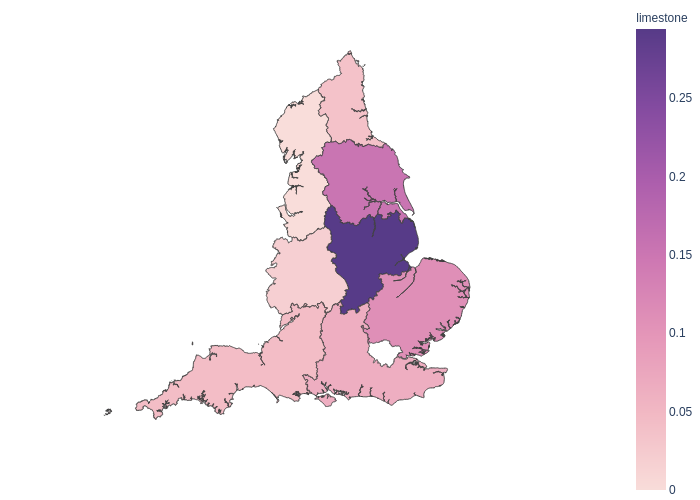
\includegraphics[width=0.45\textwidth]{limestone.png}
	\caption{Limestone}
\end{figure}
\vspace{1cm}
Data from the British Geological Survey shows a large flint deposit in the south east area where flint is featured so heavily \cite{bgs}. Sandstone covers the west of England, curving round to the North East, with the rest featuring limestone instead. The image to view this needs to be seen at a large scale, and so it provided as an appendix at the end of this paper.

In addition to these two natural resources, the derivatives of natural resources can also be seen, with the South West using a lot more brick than other areas. These observations are supported by the observations found by Hislop that brick castles are restricted to the east and south east. \cite{HislopMalcolm2016Cb:a}.

\begin{minipage}{0.45\textwidth}
	\begin{figure}[H]
		\centering
		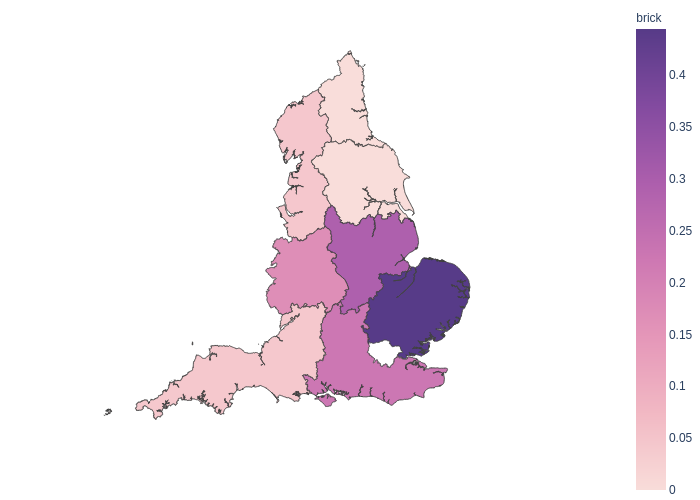
\includegraphics[width=\textwidth]{brick.png}
		\caption{Brick}
	\end{figure}
\end{minipage}
\begin{minipage}{0.45\textwidth}
	\begin{figure}[H]
		\centering
		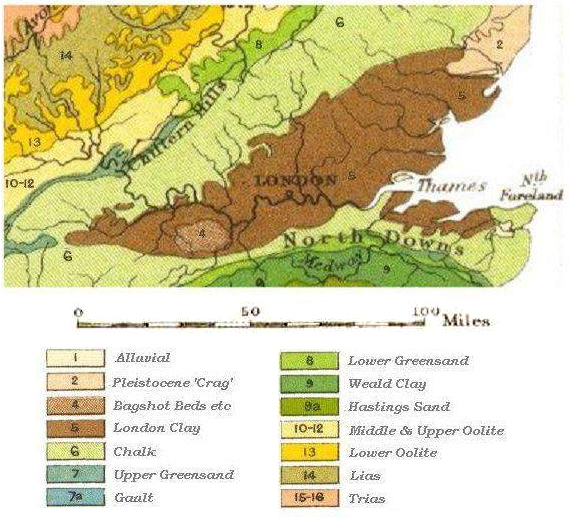
\includegraphics[width=0.9\textwidth]{Geological_map_of_London_Basin.jpg}
		\caption{London Clay}
	\end{figure}
\end{minipage}
\vspace{1cm}
\\
This is likely due to the large amount of Clay in the Thames valley, named the London Clay Formation \cite{sumbler1996london}. This can be seen in Figure 4.

Geology can also have an impact on the features the castles have, along with what they're made of. Tunnels are used in castles for seige warfare, however they have also been used for connecting sections of castles, such as the Castle of La Roche-Guyoon \cite{HislopMalcolm2016Cb:a}, where tunnels were made through the chalk. Due to the lack of machines, the ease of digging the rock the castle was built on was important for this, and this can be seen with east anglia, which has a large amount of chalk bedrock, being more common for building tunnels.

\begin{figure}[H]
	\centering
	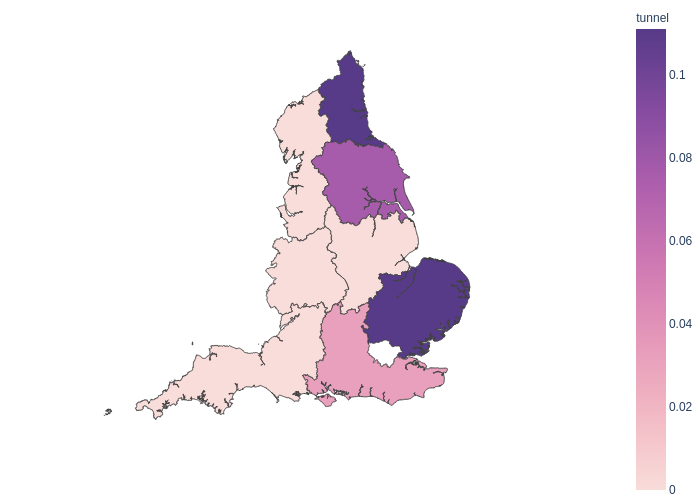
\includegraphics[width=0.45\textwidth]{tunnel.png}
	\caption{Tunnel}
\end{figure}

In addition to geology, other natural resources can impact the design of a castle, one such example of this is woodland. This is quite a difficult thing to measure as the amount of woodland varies drastically, but I was able to find a map of forest cover in 1895 \cite{trees}.

\begin{minipage}{0.45\textwidth}
	\begin{figure}[H]
		\centering
		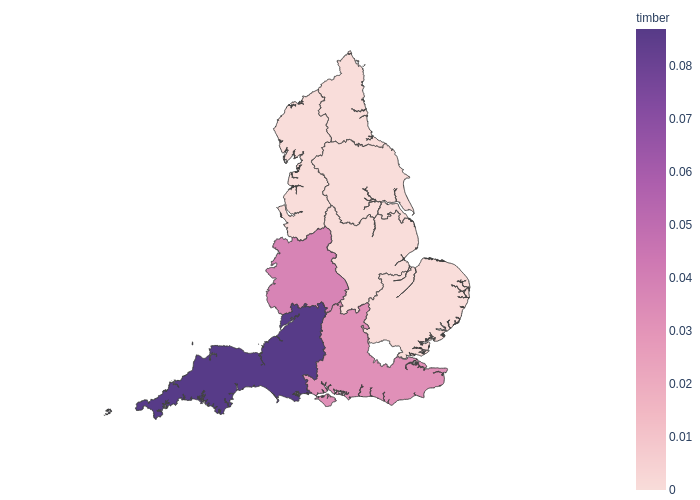
\includegraphics[width=\textwidth]{timber.png}
		\caption{Timber}
	\end{figure}
\end{minipage}
\begin{minipage}{0.45\textwidth}
	\begin{figure}[H]
		\centering
		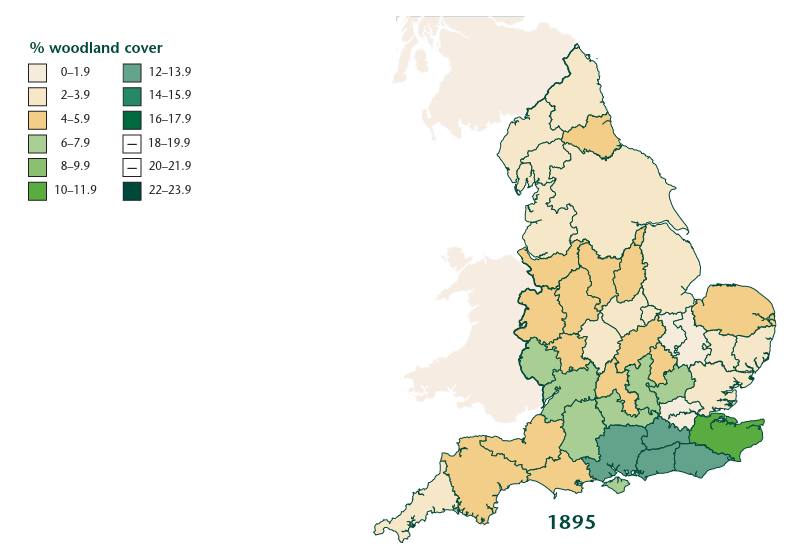
\includegraphics[width=0.9\textwidth]{forest_cover.png}
		\caption{Tree cover in 1895}
	\end{figure}
\end{minipage}

While this trend isn't a perfect match, with the South West having the most mention of Timber, but the south East having more tree cover, it does show that the areas with more forest make more use of the timber. This has been discussed in Hislop \cite{HislopMalcolm2016Cb:a}, as Richmond castle in the north of England had a superstructure of stone rather than timber due to a shortage of timber of the right quality in the area. In addition to this, the instability in the area, leading even into the 14th Century, made the use of stone, rather than wood, a good idea to avoid structural parts of the castle burning down.

One of the features most distinctly confined to one area is the use of a Basement. This trend started with Norham Castle near the Scottish border \cite{HislopMalcolm2016Cb:a} and remained in the North. This is true for a few features, the reason behind which is hypothesized to be the influence of the Palatinate of Durham \cite[p6]{HislopMalcolm2016Cb:a} as they employed master builders and master masons who worked on many of the castles in the area, and so used similar techniques.

\begin{figure}[H]
	\centering
	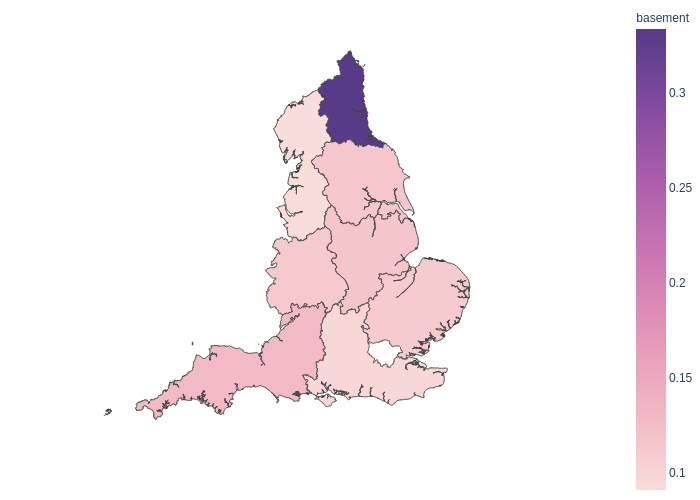
\includegraphics[width=0.45\textwidth]{basement.png}
	\caption{Basement}
\end{figure}



Near the Scottish border, castles had to defend against Border Reivers, who's main activity was stealing animals from land around the Scottish border \cite{moffat2011reivers}. It can be seen that in Northern areas, stables are more important parts of the castles, allowing to protect horses from the Reivers.

\begin{figure}[H]
	\centering
	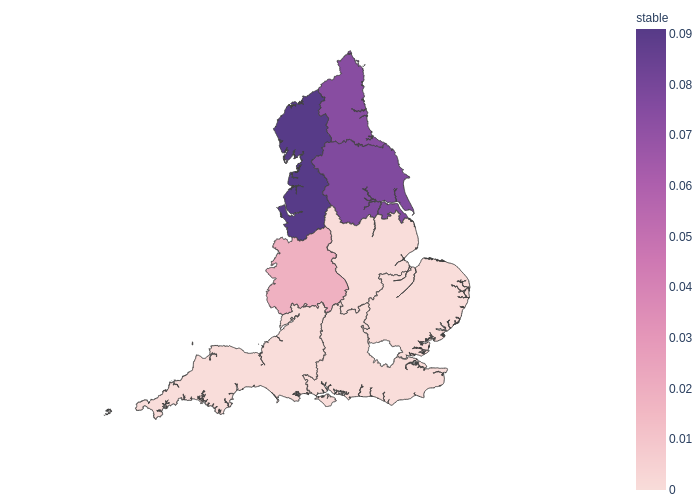
\includegraphics[width=0.45\textwidth]{stable.png}
	\caption{Stable}
\end{figure}

\section{Conclusion}

The results found could be compared with other factors in order to explain the reasons for the patterns shown. The strongest of these are the materials used for the castles as those building the castles had no choice but to use local materials, whereas specific features may change over time or for the specific challenges a castle faces. However, other features can also be observed having differences based on area for a variety of reasons, including the masons that worked on the castles and the requirements the castle has.

One limitation of this work is that it is done based on the descriptions provided in the listings, which didn't follow any specific structure. This means that features may just be neglected to be mentioned in the description for certain castles. Another limitation is the size of the dataset, with around 230 castles, the sample size isn't big enough to draw definite conclusions about areas.

Future work in this area could benefit from consultation with historians in each area as there isn't much research in how the design of castles depend on their location.



\newpage
\printbibliography

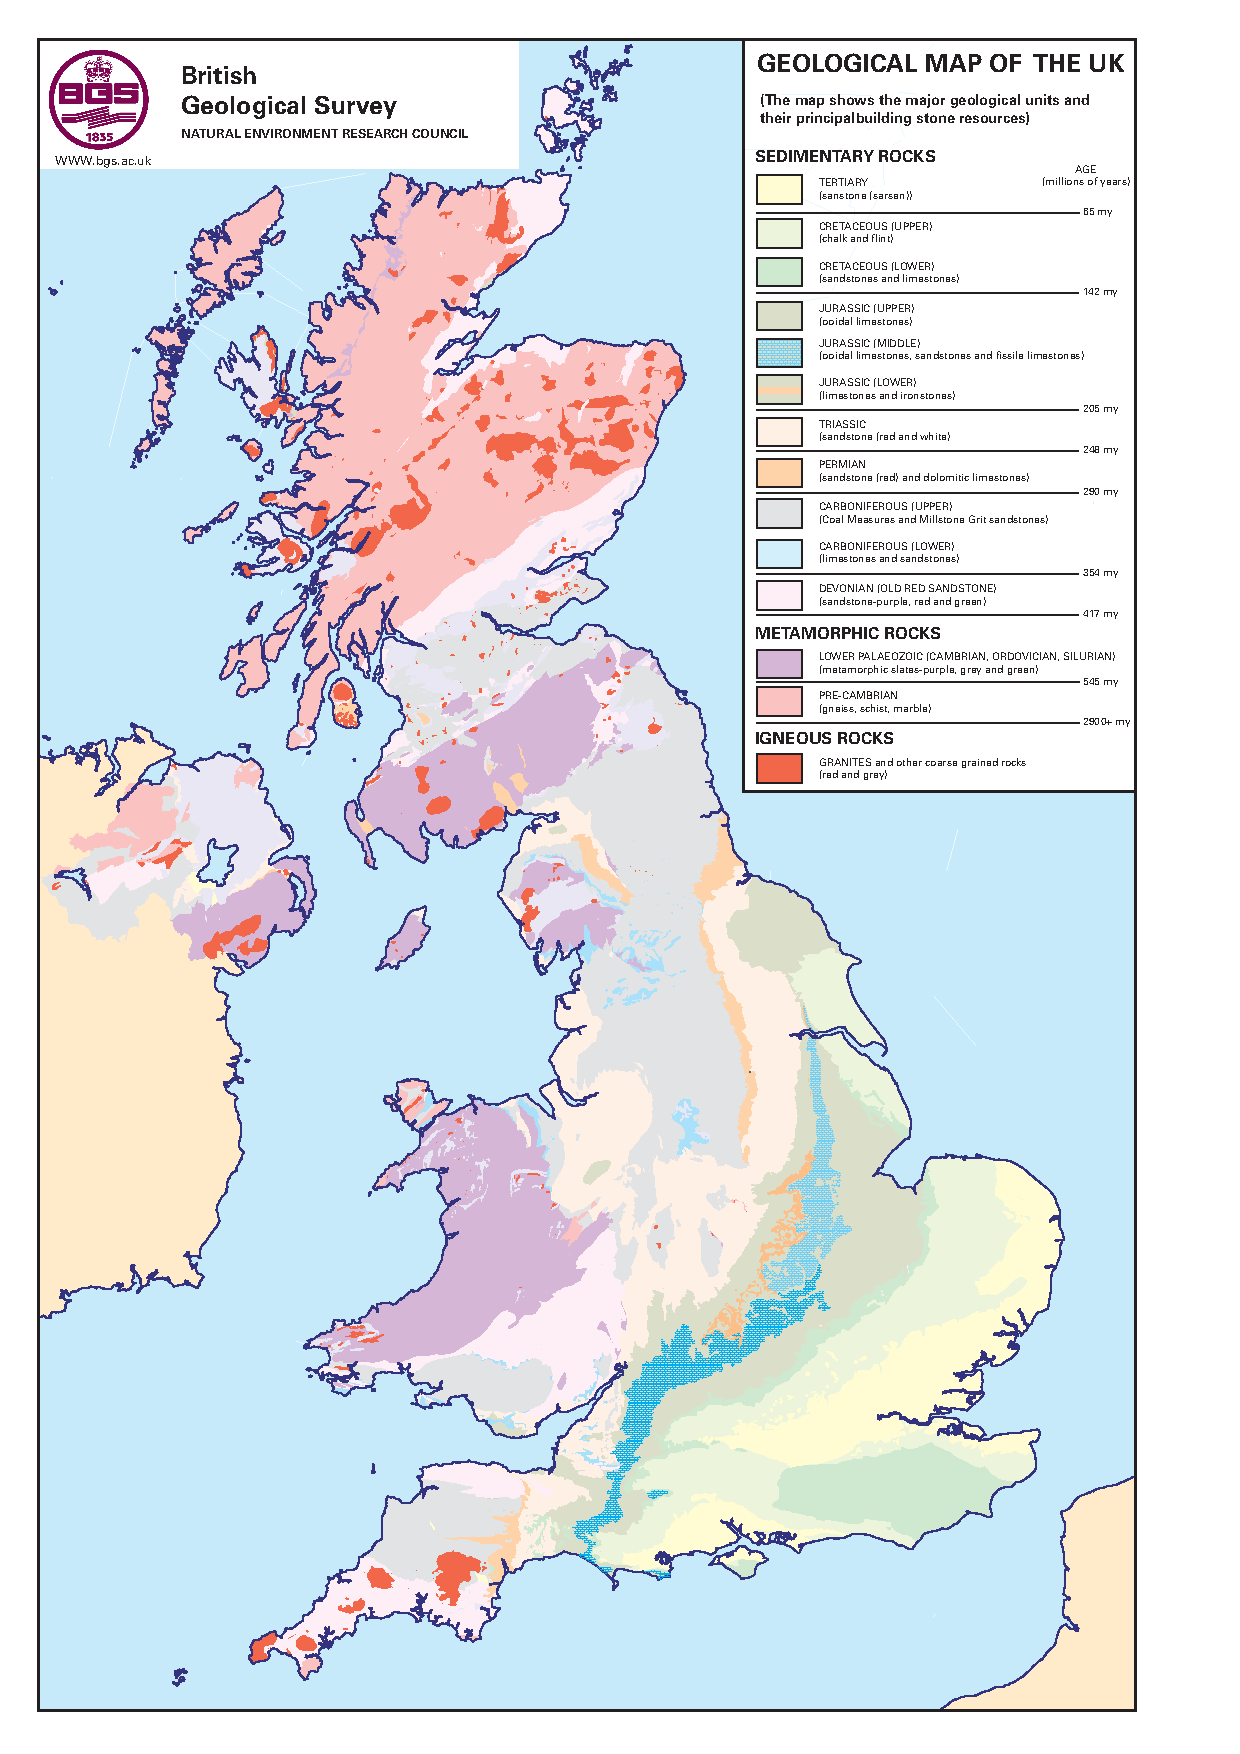
\includepdf{BGS-geological-UK-map}


\end{document}
